\section{Metode}
\subsection{Overordnet system design}
\begin{figure}[H]
    \centering
    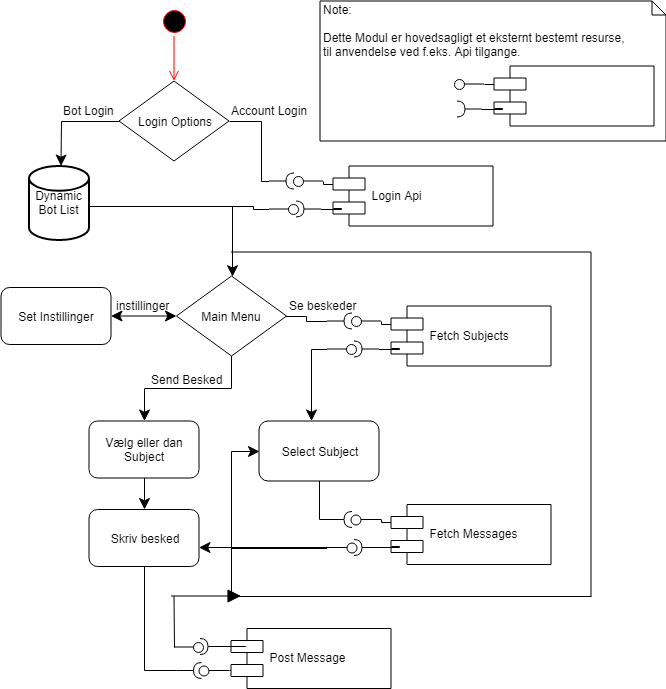
\includegraphics[width=0.85\linewidth]{Projectdoc/Assets/Illustrationer/system-diagram.png}
    \caption{System aktiverings diagram}
    \label{fig:sysdiagram}
\end{figure}

Systemet beskrevet ved [Figur \ref{fig:sysdiagram}] er hovedsageligt designet efter et user activated action event flow. 
Dette vil sige at alle systemets aktiviteter er baseret på en brugers aktive handlinger, og kan derved styres fra et centralt sted. Her tales om enten brugerens egen device, eller en central system server, der kun responder på brugerens kommandoer.
En af de stører fordele ved at have en central server, i modsætning til brugerense device for håndtering, er den markant stører mulighed for lokalt data. På en central server er der mulighed for at forebygge heavy-load og f.eks. loade, samt gemme (som en slags cashe), alle beskeder for en specifik tråd, inden brugeren faktisk beder om dennes indhold. Derved kan man benytte serverens idel-state til at aktivt forebygge aktiviteter, og derved minske fremtidig load time.



En central server trods dens eventuelle positive effekter, er dog også et generelt stører sikkerhedsbrug. F.eks. Kunne en sådan server leake generelle lagerede informationer, eller lige frem enten blive overvåget for kommunikation, samt blive spæret som en helhed. Dette vil selvfølgelig også kunne ske for den enkelte bruger, men disse ville i sådanne tilfælde også kun påvirke den enkelte, og ikke systemet som en helhed. Grundet disse negative effekter for en central server, der generelt berører brugerens sikkerhed, vil den mest optimale løsning for projektets sikre kommunikation være at anvende brugernes enkelte devices til system håndtering.

% Central server, pros/cons

\subsection{Teori}

% Hvad er Api struktur ?

% Hvad er socket kommunikation ?

% Dynamic updating / Databaser ?



\subsection{Detaljeret system design}
% Hvordan skal forum strukturen være ?
% ^ sammenkædningen af beskeder.
% Hvordan kan man sikre en fornuftig køre tid ? (Undgå 10000 undersøgelser for at finde én kommentar)

% - Database dynamisk

% - 